\documentclass[10pt, letterpaper]{article}

\usepackage{tikz} 
\usepackage{pgfplots}
\pgfplotsset{compat=1.9}
\usetikzlibrary{arrows,shapes,automata,backgrounds,petri,fit,decorations.pathmorphing, calc}

\begin{document}
\begin{center}
  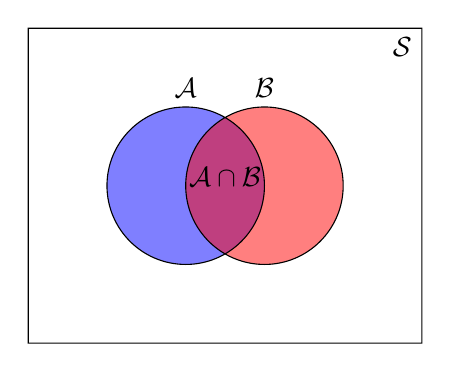
\begin{tikzpicture}[fill=lightgray]
    % left hand
    \scope
            (-2,-2) rectangle (2,2)
            (1,0) circle (1);
      \fill[blue, opacity = .5] (0,0) circle (1);
    \endscope
    
    % right hand
    \scope
            (-2,-2) rectangle (2,2)
            (0,0) circle (1);
      \fill[red, opacity = .5] (1,0) circle (1);
    \endscope
  
    % outline
    \draw (0,0) circle (1) (0,1)  node [text=black,above] {$\mathcal{A}$}
          (1,0) circle (1) (1,1)  node [text=black,above] {$\mathcal{B}$}
          (1,0) circle (1) (1,1)  node [text=black,below, xshift = -.50cm, yshift = -.65cm] {$\mathcal{A \cap B}$}
          (-2,-2) rectangle (3,2) node [text=black,below, xshift = -.25cm] {$\mathcal{S}$};
  \end{tikzpicture}
\end{center}
\end{document}